\chapter{Genomic prediction: some caveats}\index{genomic prediction!caveats}

In the early 2010s, Turchin and
colleagues~\cite{Turchin-etal-2012}\footnote{{\it Michael\/} Turchin,
  not {\it Peter\/} Turchin of UConn's EEB department.} studied the
association between variation at SNP loci and height in humans. They
showed that both individual alleles known to be associated with
increased height and in genome-wide analysis are elevated in northern
European populations compared to populations from southern
Europe. They argued that these differences were consistent with weak
selection at each of the loci~($s \approx [10^{-3}, 10^{-5}]$) rather
than genetic drift alone.

\subsection*{Allele frequency comparisons}

Turchin et al.\ used allele frequency estimates from the Myocardial
Infarction Genetics consortium~(MIGen)~\cite{MIGen-2009} and the
Population Reference Sample~(POPRES)~\cite{Nelson-etal-2008}. For the MIGen
analysis, they compared allele frequencies in 257 US individuals of
northern European ancestry with those in 254 Spanish individuals at
loci that are known to be associated with height based on GWAS
analysis\footnote{See Turchin et al. for details.} and found
differences greater than those expected based on 10,000 SNPs drawn at
random and matched to allele frequencies at the target loci in each
population. They performed a similar analysis with the POPRES sample
and found similar results.

Turchin et al. were aware that the association could be spurious if
ancestry was not fully accounted for in these analyses, so they also
used data collected by the Genetic Investigation of ANthropometric
Traits consortium (GIANT)~\cite{LangoAllen-etal-2010}.\footnote{This
  includes the GWAS on height that I mentioned in the last lecture.}
They noted that ``control'' SNPs used in the preceding analysis,
i.e., the 10,000 SNPs drawn at random from the genome, with a tendency
to increase height in the GIANT analysis also tended to be more
frequent in the northern European sample.

They compared the magnitude of the observed differences at the most
strongly associated 1400 SNPs with what would be expected if they were
due entirely to drift and what would be expected if they were due to a
combination of drift and selection. A likelihood-ratio test of the
drift alone model {\it versus\/} the drift-selection model provided
strong support for the drift-model.

\section*{Second thoughts}

\subsection*{Within sample stratification}\index{genomic prediction!sample stratification}

This all seems very promising, but a word of caution is in order. Berg
et al.~\cite{Berg-etal-2018} re-examined these claims using new data
available from the UK
Biobank~(\url{https://www.bdi.ox.ac.uk/research/uk-biobank}), which
includes a host of information on individual phenotypes as well as
genome-wide genotypes for the 500,000 individuals included in the
sample.\footnote{Although all of the samples are from the UK, one of
  the data sets Berg et al.~\cite{Berg-etal-2018} studied included
  individuals of European, but non-UK, ancestry.} They failed to
detect evidence of a cline in polygenic scores in their
analysis~(Figure~\ref{fig:UK-biobank}).

\begin{figure}
  \begin{center}
    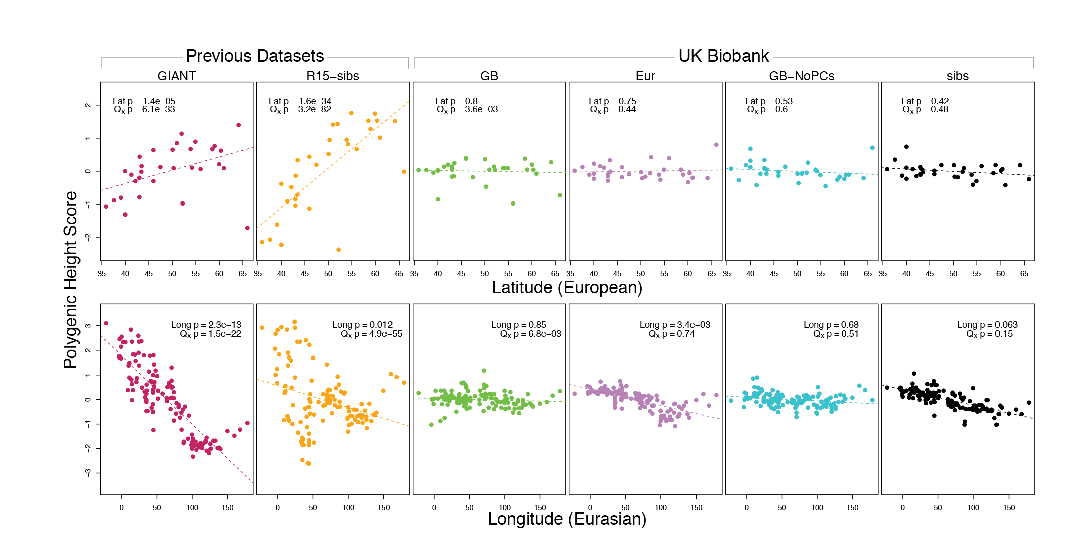
\includegraphics[width=\textwidth]{UK-biobank.eps}
  \end{center}
  \caption{Polygenic score as a function of latitude and longitude for
    several different GWAS data sets. Each vertical column corresponds
  to a different data source. Notice that all of the UK Biobank
  samples fail to show either a latitudinal or a longitudinal cline in
  polygenic height score~(from \cite{Berg-etal-2018}).}\label{fig:UK-biobank} 
\end{figure}

In thinking about this result, it's important to understand that Berg
et al.~\cite{Berg-etal-2018} did something a bit different from what
we did, but it's exactly what you'd want to do if polygenic scores
worked. They estimated polygenic scores from each of the data sets
identified in the figure. Then they used those scores to estimate
polygenic scores for a new set of samples derived from the 1000
Genomes and Human Origins projects.\footnote{See Berg et
  al.~\cite{Berg-etal-2018} for details.} Since they did the same
thing with all of the data sets, this difference from what we did
doesn't account for the differences among data sets. As Berg et
al. dug more deeply into the data, they concluded that all of the data
sets ``primarily capture real signals of association with height'' but
that the GIANT and R-15 sibs data sets, the ones that show the
latitudinal (and longitudinal in the case of GIANT) associations do so
because the estimated allelic effects in those data sets failed to
fully remove confounding variation along the major geographic axes in
Europe.

The Berg et al. analysis illustrates how difficult it is to remove
confounding factors from GWAS and genomic prediction
analyses. Turchin et al. are highly skilled population geneticists. If
they weren't able to recognize the problem with stratification in the
GIANT consortium data set, all of us should be concerned about
recognizing it in our own. Indeed, I wonder whether the stratification
within GIANT would ever have come to light had Berg et al. not had
additional large data sets at their disposal in which they could try
to replicate the results.

\subsection*{Difficulties extrapolating polygenic scores}

In one way the Berg et al. results are actually encouraging. They
estimated effects in one set of data and used the genomic regressions
estimated from those data to predict polygenic scores in a new data
pretty successfully. Maybe it's difficult to be sure that the
polygenic scores we estimate are useful for inferring anything about
natural selection on the traits they predict, but if we could be sure
that they allow us to predict phenotypes in populations we haven't
studied yet, they could still be very useful. Can we trust them that
far?

Unfortunately, the answer appears to be ``No.'' Yair and
Coop~\cite{Yair-Coop-2021} recently studied the relationship between
phenotypic stabilizing selection and genetic differentiation in
isolated populations. They showed that even in a very simple model in
which allelic effects at each locus are the same in both populations,
polygenic scores estimated from one population may not perform very
well in the other. Interestingly, as you can see in
Figure~\ref{fig:yair-coop-predictions}, the stronger the selection and
the more strongly allelic differences influence the phenotype, the less
well genomic predictions in one population work in the other.

\begin{figure}
  \begin{center}
    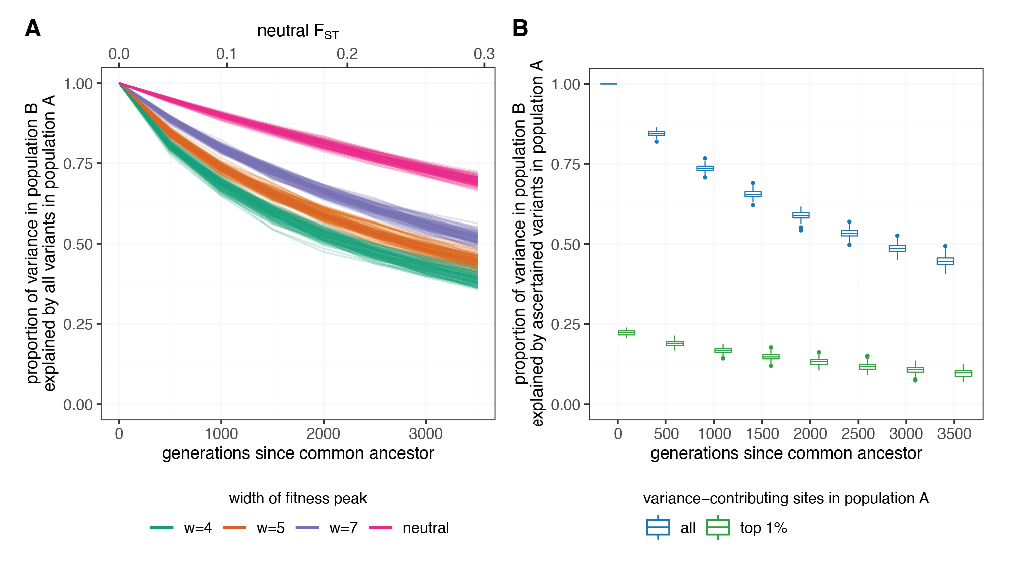
\includegraphics[width=\textwidth]{yair-coop-predictions.eps}
  \end{center}
  \caption{Polygenic score as a function of latitude and longitude for
    several different GWAS data sets. Each vertical column corresponds
  to a different data source. Notice that all of the UK Biobank
  samples fail to show either a latitudinal or a longitudinal cline in
  polygenic height score~(from~\cite{Yair-Coop-2021}).}\label{fig:UK-biobank} 
\end{figure}

That seems paradoxical, but interestingly it's not too difficult to
understand if we think about what happens when we combine stabilizing
selection with geographical isolation.\footnote{And the fun thing for
  me about this is that we get to finish out the course by returning
  to a paper I wrote with my first master's student more than 30 years
  ago.} First, let's remind ourselves of a fundamental property of
polygenic variation: Different genotypes can produce the same
phenotype. Figure~\ref{fig:redundancy}, which you've seen before,
illustrates this when three loci influence the trait. While there is
only one genotype that produces the dark red phenotype and only one
that produces the white phenotype, there are four genotypes that
produce the light red phenotype, four that produce the medium dark red
phenotype, and six that produce the medium red phenotype. Goldstein
and Holsinger~\cite{Goldstein-Holsinger-1992} called this phenomenon
{\it genetic redundancy}.\index{genetic redundancy} As you can
imagine, the number of redundant genotypes increases dramatically as
the number of loci involved increases.\footnote{If the allelic effects
  are strictly additive, the number of genotypes corresponding to the
  intermediate phenotype is $2N \choose N$ where $N$ is the number of
  loci. For $N=10$, ${2N \choose N} = 184,756$. For $N=100$, ${2N \choose
  N} = 9.05 \times 10^{58}$.}

\begin{figure}
  \begin{center}
    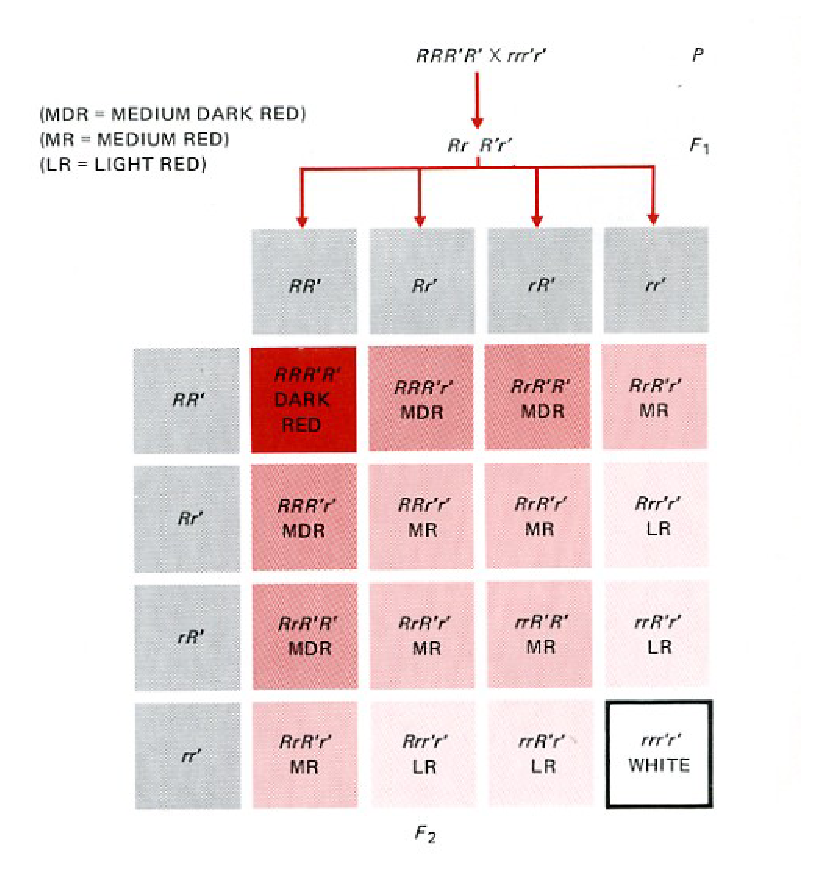
\includegraphics[width=10cm]{Nilsson-Ehle.eps}
  \end{center}
  \caption{Results from one of Nilsson-Ehle's crosses illustrating
    polygenic inheritance of kernel color in wheat~(from {\tt
      http://www.biology-pages.info/Q/QTL.html}, accessed 9 April 2017).}\label{fig:redundancy}
\end{figure}

Why does this redundancy matter? Let's consider what happens when we
impose stabilizing selection on a polygenic trait, where
$$
w(z) = \mbox{exp}\left(\frac{-(z - z_0)^2}{2V_s}\right) \quad ,
$$
where $z_0$ is the intermediate phenotype favored by selection, $z$ is
the phenotype of a particular individual, and $V_s$ is the variance of
the fitness function. If selection is weak ($V_s = 115.2$), then the
relative fitness of a genotype 1 unit away from the optimum is 0.9957
while that of a genotype 8 units away is only 0.7575. If 16 loci
influence the trait, there are 601,080,390 genotypes that produce the
optimum phenotype and have the same fitness. There are another
1,131,445,440 genotypes whose fitness within one percent of the
optimum. Not only are there a lot of different genotypes with roughly
the same fitness, the selection at any one locus is very weak.

Now suppose these genotypes are distributed in a large, continuous
population. Because selection is pretty weak and because mating is
primarily with close neighbors, allele frequency changes at each locus
will be close to what they would be if the loci were neutral. The
result is that the genetic correlation between individuals drops off
rapidly as a function of the distance between
them~(Figure~\ref{fig:isolation-by-distance}). Notice that in the
simulation illustrated individuals separated by more than about 20
distance units are effectively uncorrelated. That means that their
genotypes are essentially random with respect to one another, even
though their phenotypes are similar because of the stabilizing
selection. 

\begin{figure}
\begin{center}
\resizebox{!}{10cm}{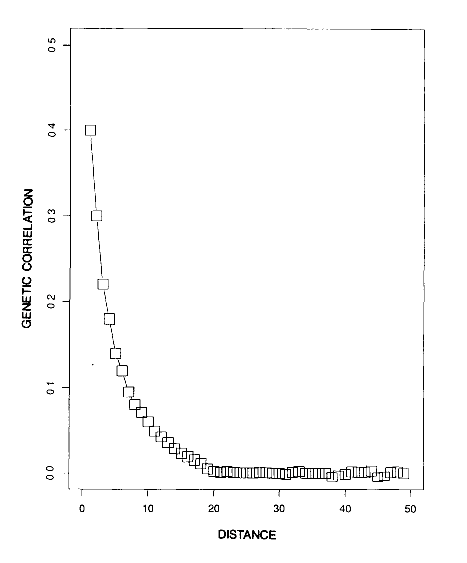
\includegraphics{isolation-by-distance.eps}}
\end{center}
\caption{Isolation by distance with weak
  selection~(from~\cite{Goldstein-Holsinger-1992}).}\label{fig:isolation-by-distance}
\end{figure}

Now think about what that means for polygenic scores. Imagine that we
sampled two ends of a large, continuously distributed population. To
make things concrete, let's imagine that the population is distributed
primarily North-South so that our samples come from a northern
population and a southern one. Now imagine that we've done a GWAS in
the northern population and we want to use the genomic predictions
from that population to predict phenotypes in the southern
population. What's going to happen?

The genotypes in the southern population will be a random sample from
all of the possible genotypes that could produce the same optimal
phenotype (or something close to the optimum) and that sample will be
independent of the sample of genotypes represented in our northern
population. As a result, there are sure to be loci that are useful for
predicting phenotype in the northern population that aren't variable
in the southern population, which will reduce the accuracy of our
genomic prediction. That's precisely what Yair and Coop
show.\footnote{Although their results go much farther than Goldstein
  and Holsinger who did their simulations long before anyone was
  thinking about GWAS, much less genomic prediction and polygenic
  scores.}

In short, it's to be expected that genomic predictions will be useful
only within the population for which they are constructed. They can be
very useful in plant and animal breeding, for example, but any attempt
to use them in other contexts must be alert to the ways in which
extrapolation from one population to another will be problematic.

